The data handling is organised into 3 sections: The first being a MongoDB data-store for handling all the incoming data from the flowers, the second being the dashboard for visualising the data available in the data-store and the last being a central server that communicates with a lora-module via serial-port, parsing and saving the lora packets and also acting as a web-server to the dashboard.

\subsection{MongoDB Data store}
% Quick intro to MongoDB (No-SQL)
MongoDB is a No-SQL database that provides an expressive query language and flexible data-store that allows iteration of data models. It is a highly efficient database that supports millions of operations per sec and can handle petabytes of data as well being able to scale (grow) horizontally with support for database clusters.

% Benefits of MongoDB (Rapid prototyping)
This rich feature set provided us with a strong foundation as a data-store for the sunflowers for two main reasons. Firstly, during the development stage, it provided us with a medium for rapid prototyping as we were able to rapidly change the schema of the data that was being stored and 
% Scalability and distributed nature which can support distributed sunflowers
due the distributed and highly scalable nature of MongoDB; It is theoretically possible for us to scale this data-store to support thousands of sunflowers.

\subsection{Dashboard}
% Brief intro to the dashboard as a valuable tool for analytics
The dashboard acts as an operator user-interface for navigating the data in the MongoDB data-store. One of the functionalities we encoded into it is support for analytics on the Sun flower data, this is illustrated in figure \ref{figure:home} where we aggregated data on the temperature and humidity.
\begin{figure}
	\centering
	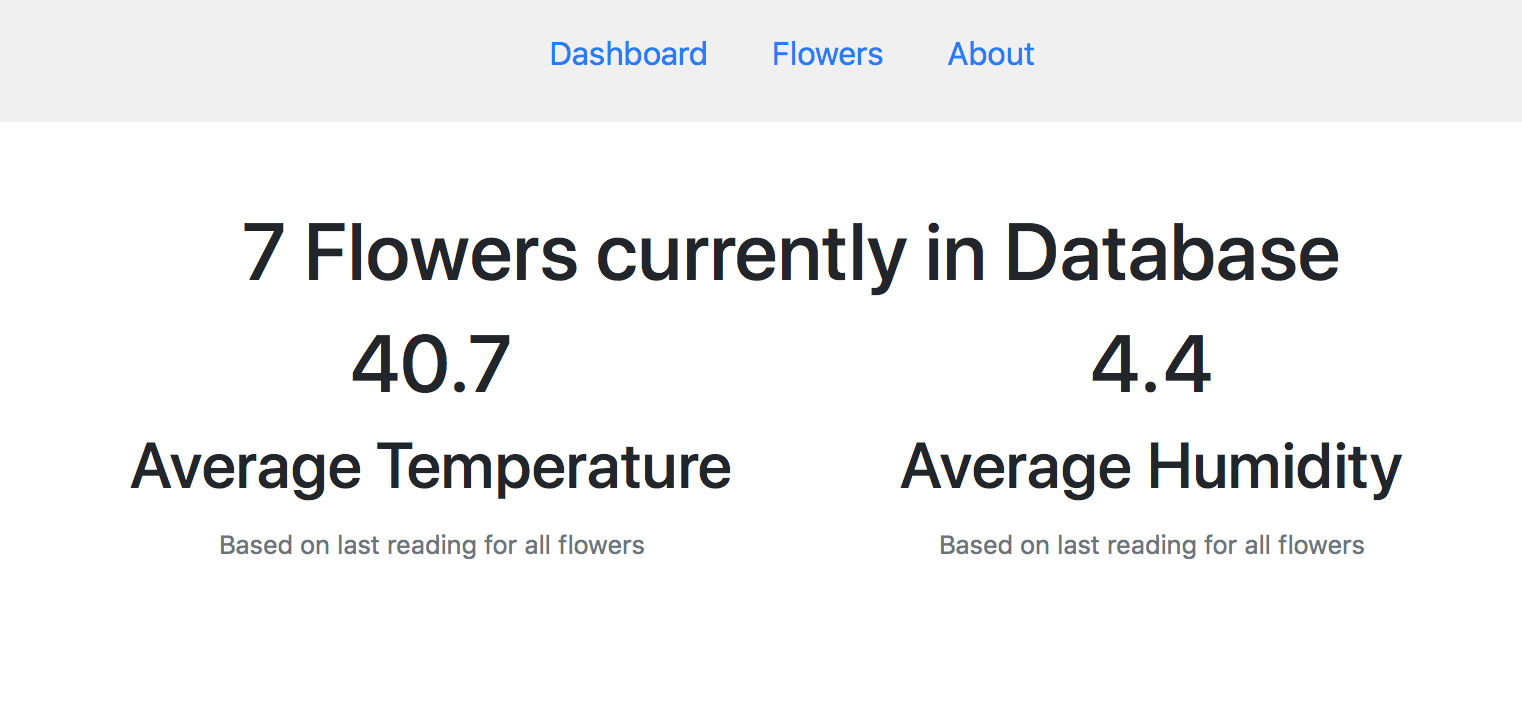
\includegraphics[width=\linewidth]{home}
	\caption{Homepage for the dashboard}
	\label{figure:home}
\end{figure}
\begin{figure}
	\centering
	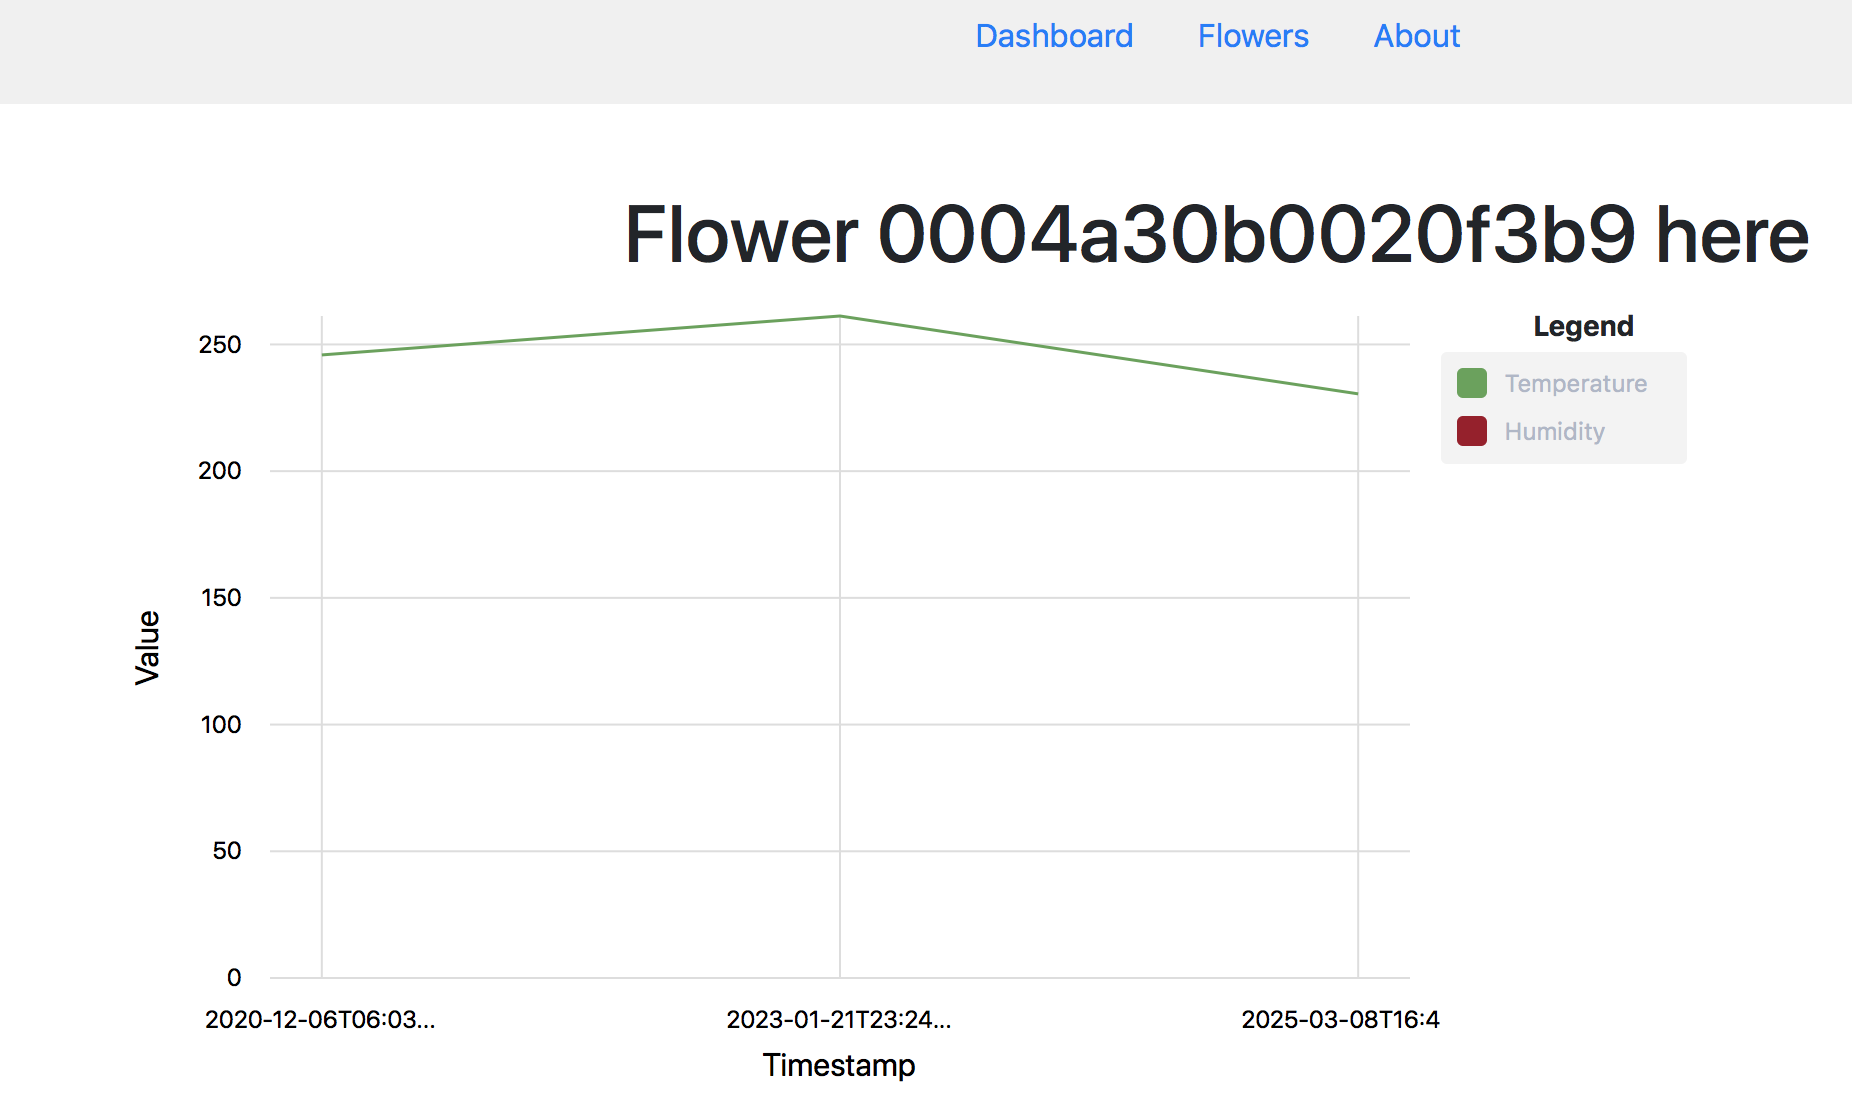
\includegraphics[width=\linewidth]{flowers}
	\caption{Sample detail page for a SunFlower}
	\label{figure:flower}
\end{figure}

% Quick intro into the tech behind the dashboard
The dashboard is built using web-technologies of which are \href{www.angular.io}{AngularJS} for the architecture and \href{https://swimlane.github.io/ngx-charts/}{Ngx-Charts} for the visualisations. The dashboard supports single-page apps and by default offline mode; highlighting the strong technologies used for the project.

% Currently supports one way communication i.e Flower => Server => Dashboard but support for bilateral comms could be added in the future
Currently the dashboard only receives data from the central server as data currently flows from the sun-flowers to the server and then to the dashboard. In the future, bilateral communication could be added; In figure \ref{figure:flower}, the sample page for a sun-flower is shown there, a sample feature that could be added would be a button to shutdown the flower where this command propagates from the dashboard to the central server and then to the sun-flower.



\subsection{Central Server}
%TODO - Quick intro in the tech behind the server (highly scalable and asynchronous in nature)
%TODO - Functionality of the server: Node serial port communication and parsing, saving to disk, processing the data for analytics
%TODO - REST API exposed which can be used by mobile apps, web-apps etc
%TODO: Include an image of the entire pipeline